\documentclass[12pt]{article}
\usepackage[a4paper, portrait, margin=1cm, right=1cm]{geometry}
\usepackage{fontspec}
\usepackage{graphicx}
\usepackage[fleqn]{amsmath}
\usepackage{indentfirst}

\graphicspath{./graphics/}
\setmainfont[Ligatures=TeX]{Linux Libertine}

\title{Информационные технологии. Лекция 08. Роевой интеллект}
\author{Студент группы 2305 Макурин Александр}
\date{10 апреля 2023}
\begin{document}
\maketitle
$f: X\rightarrow Y$ — найти некую функцию отображаения.

$y_i$ — решение

$\overline{y_i} = f(x_i)$

$Err = \sum_i(\overline{y_i} - y_i)^2$

$f = \arg \min Err$ — задача оптимизации.

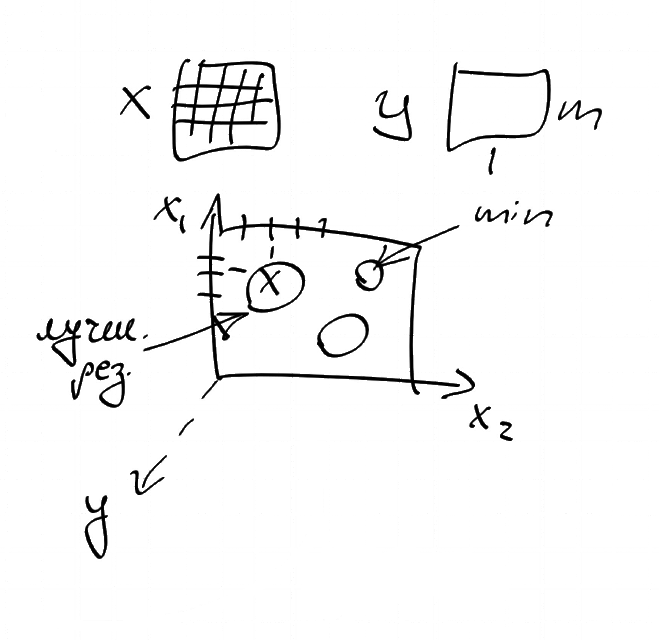
\includegraphics[width=0.5\textwidth]{graphics/pic01.png}

Или, упрощённо, нужно найти экстремум:

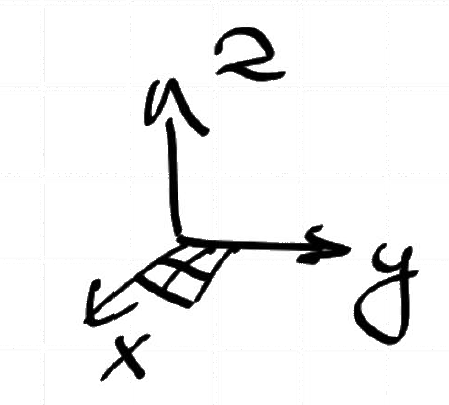
\includegraphics[width=0.2\textwidth]{graphics/pic02.png}

$f(x, y, z) = \sum \begin{cases}
        0, \text{нет} \\
        1, \text{есть}
    \end{cases}$

$(x \times y) \times z$

Попарное прохождение по координатам.

Рассмотрим $|S| > 1$ (роевой интеллект). $S$ — популяция.

\section{Общая концепция}
\begin{enumerate}
    \item Элементы — частицы.
          \begin{align*}
               & S_{ij} \pm S_{ij+1} \\
               & S_{ij} \neq S_{R_j} \\
               & S_{iT} = S_{RT}
          \end{align*}
    \item $S = \cup S_{sub}$ — стратефикация по:
          \begin{itemize}
              \item поведению
              \item связи
          \end{itemize}
    \item Децентрализовано, по принципу стаи
    \item $\exists$ косвенный обмен информации: $S_{ij} = f(S_{ij-1}, X_{ij}, \{M\})$
    \item $S_{ij} \simeq (position)$
    \item $S_{ij} \neq S_{ij+1}$
    \item $\min$
    \item $V$ — ?
\end{enumerate}

Пример уменьшения ошибки методом градиентного спуска:

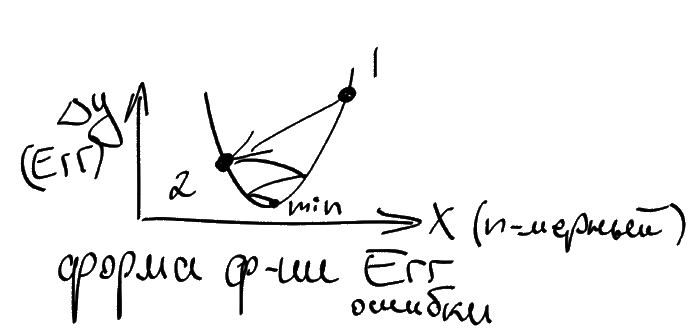
\includegraphics[width=0.5\textwidth]{graphics/pic03.png}

При такой оптимизации можно попасть в локальный минимум функции и не получить оптимального решения.

Форма функции оценки (ошибки) зависит от целевой задачи и моделируемого аппарата.

\section{Алгоритм Boids (1986 г) — начало роевого интеллекта}
\begin{enumerate}
    \item При перемещении из определённой точки A в неопределённую точку B: \\
          $x_{ij} = \dfrac{\sum{x_j}}{|x_j|}$ — пытается находится в центре
    \item $V = \dfrac{\sum V_j}{|V_j|}$ — усредняется
    \item $\rho(i, e) \geq \text{const}$ $M(x_j, V_{j - 1})$. $\rho$ — расстояние.
\end{enumerate}

\section{Particle Swarm Optimization (PSO)}

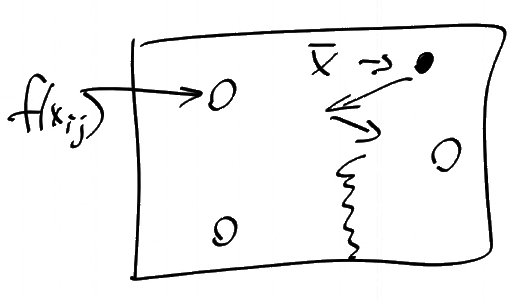
\includegraphics[width=0.5\textwidth]{graphics/pic04.png}
\begin{enumerate}
    \setcounter{enumi}{-1}
    \item $S = \{S_1, ..., S_n\}$ \\
          $S_i = <x_{ij}, V_{ij}, \overline{X_i}>$. $\overline{X_i}$ — лучшее целевое значение, когда-либо достигнутое этим агентом. $X_i = \arg \min \{x_{ij}\}_0$.
    \item Есть пространство, случайным образом кидаются элементы, выбираем $\overline{X}$.
    \item Для каждой точки ищется $f(x_{ij})$ оптимальное для ${i}_j$ $\overline{x_j}$.
    \item $x_{ij+1} = x_{ij} + V_{ij+1}$ \\
          $V_{ij+1} = \omega V_{ij} + \alpha_1 (\overline{x_i} - x_i) \times U + \alpha_2 (\overline{x_j} - x_i) \times U$ \\
          $\overline{x_j}$ — квазиглобальный экстремум. $\omega V_{ij}$ — учёт предыдущих значений. $\overline{x_i} - x_i$ — когнитивная составляющая (насколько верить самим себе). $\overline{x_j} - x_i$ — социальная составляющая. $\omega, \alpha_1, \alpha_2$ — гиперпараметры. $U$ — случайная величина, имеющая нормальное распределение на $[a, b]$ (определяет стохастический характер, нет уверенности, что алгоритм сойдётся). \\
          Экспериментально выяснено, что $\omega = 0.7298$. \\
          $[a, b] = [0, 1]$ — стандартно. \\
          $V_{ij + 1} = \omega V_{ij} + \alpha_1(\overline{x_i} - x_i) U + \sum Trust t_{ik} (\overline{x_l} - x_i)U$
\end{enumerate}

\section{Подробно про муравьиный алгоритм}
$S = <X, T>$ $M = (F, R)$

$t^e_{ij} = \begin{cases} 0 \\ 1 \end{cases}$

\begin{enumerate}
    \item $F = |\text{верш.}|(\text{const})$
    \item $f(x_{ij}) \Rightarrow \overline{x_j}$
    \item $aT_{kl} = \begin{cases}
                  (\dfrac{\gamma}{f(x_{ij})})^\mu \text{, $\gamma$, $\mu$ — гиперпараметры} \\
                  0
              \end{cases}$ \\
          $T_{kl}^{j + 1} = T_{kl}^j + \Delta$ \\
          $\overline{T_{kl}} = min(T_{kl}^{j+1} \lambda, T_{k_1k_2}^{max})$
    \item $\theta = \rho T_{kl}^j + \Delta$ \\
          $T_{kl}^j = \begin{cases}
                  \theta, \theta \geq T_{min} \\
                  T_{min}, \theta < T_{min}
              \end{cases}$ \\
          $\rho$ — показатель испарения (гиперпараметр), $\theta$ — гиперпараметр.
    \item $p_m = \begin{cases}
                  \dfrac{(T^{km})^\alpha \eta(r_{km})^\beta}{\sum(T_{kz})^\alpha \eta (r_{kz})^\beta} \text{ — нормирование относительно ещё не посещённых вершин} \\
                  0 \text{, th = 1}
              \end{cases}$
\end{enumerate}

\section{Адекватность поведения при обходе графа. Алгоритм светлячка}
$F_i \text{ re (реагирует) } F_{e_y}$

$S, f(x_{ij})$, $x_{ij}$ — свечение.

\begin{enumerate}
    \item Случайное распределение
    \item Определение самого яркого $f(x_{ij}) \Rightarrow \overline{x_j}$
    \item Все стремятся к ярчайшим
          $x_{ij+1} = x_{ij} + \delta(x_{ij}, x_{kj})(x_{kj}-x_{ij}) + \alpha U$. $\delta(a, b)$ — притягательность светлячка.\\
          $\delta = \begin{cases}
                  \dfrac{\beta}{1 + \gamma r}, \overline{x_k} \geq \overline{x_j} \\
                  0, \overline{x_k} < \overline{x_j}
              \end{cases}$ \\
          $\beta, \gamma, \alpha$ — гиперпараметры. Если $\delta = 0 \Rightarrow$ формула самого притягательного светлячка.
\end{enumerate}

Самый светлый движется хаотически.

Вариация алгоритма ведущий — ведомый.

\end{document}